\lab{Algorithms}{IVP Methods}{IVP Methods}
\label{lab:IVP}

\objective{Implement several basic numerical methods for initial value problems, and use them to study harmonic oscillators.}

\section{Methods for initial value problems}
Consider the initial value problem 
\begin{align*}
y' &= f(x,y),\,\, a \leq x \leq b, \\
y(a) &= y_0,
\end{align*}
where $f$ is a continuous function. A solution is a continuously differentiable function $y(x)$ that satisfies the equation $y' = f(x,y)$ on the interval $[a,b]$ and for which $y(a) = y_0$.  

There are many initial value problems (IVPs) where it is impossible to find a closed form (analytic) expression for the solution. 
For other IVPs there is a closed form expression for the solution, but it may be difficult to interpret. 
In either case, we can usually make good use of various methods of numerical approximation to study the solution. (It is still important to know mathematically that a solution exists, even when we cannot find an explicit solution!)


Consider the initial value problem 
\begin{align*}
y'(x) &= \sin y(x), \\
y(0) &= y_0.
\end{align*}
This IVP does have solution, which is given implicitly by 
\[x = \ln \left|\frac{\cos y_0 + \cot y_0}{\csc y + \cot y} \right|.\]
In this case, to understand the general solution it helps to use an IVP solver to plot the integral curves for some initial values. It is easy to show that this differential equation has constant solutions $y_n(x) = n \pi, n \in \mathbb{N}$. Knowing this, and after plotting several integral curves (see Figure \ref{ivp:int_curves} ), it is obvious how solutions of this IVP will behave.

\begin{figure}
\centering
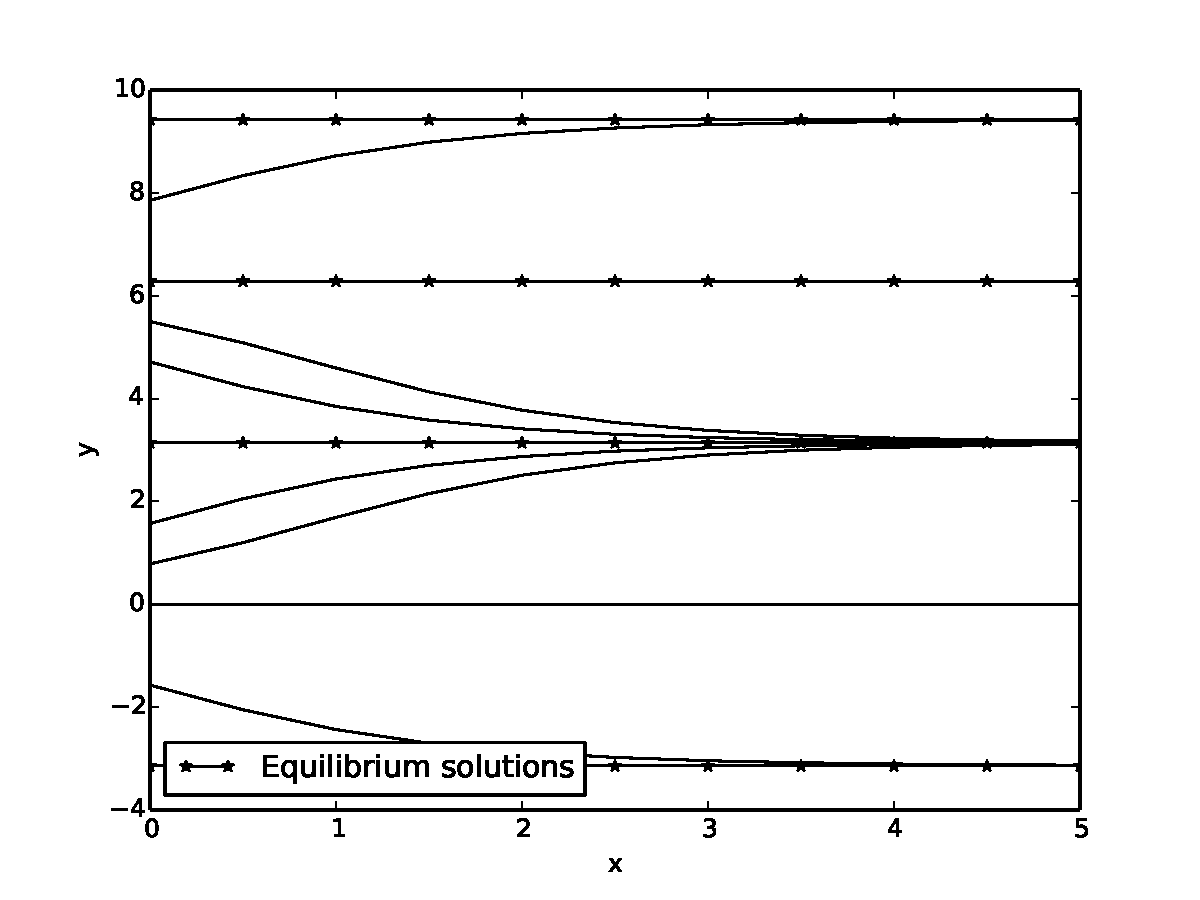
\includegraphics[width=\textwidth]{Fig2.pdf}
\caption{Several integral curves for the differential equation $y' =\sin y$, using the python solver \li{dopri5}. }
\label{ivp:int_curves}
\end{figure}



Numerical methods for solving intial value problems require us to approximate the solution on a set of grid points $a = x_0< x_1<\hdots< x_n = b$ in our interval.  For simplicity we will assume that each of the $n$ subintervals $[x_{i-1},x_i]$ has equal length $h = (b-a)/n$. $h$ is called the \textit{step size}. We then look for values $y_0,y_1, \hdots, y_n$ that approximate our solution ( so $y_i \approx y(x_i)$).  

For a fixed value of $i$, $ 1 \leq i \leq n$, Taylor's theorem says that 
\begin{align*}
y(x_{i+1}) &= y(x_{i}) + h y'(x_i) + \frac{h^2}{2} y''(\xi_i)\text{ for some }\xi_i \in [x_i,x_{i+1}].
\end{align*}
For small values of $h$ the quantity $\frac{h^2}{2} y''(\xi_i)$ will be negligible and so we will have
\begin{align*}
y(x_{i+1}) &\approx y(x_{i}) + h y'(x_i)  ,\\
&\approx y(x_{i}) + h f(x_i,y(x_i)).
\end{align*}
This approximation leads to a first order ($\mathcal{O}(h^1)$) method called Euler's method: Let $y_0 = y(a)$, and for $i = 0, 1, \hdots, n-1$, let $y_{i+1} = y_i +hf(x_i,y_i)$. 
% \begin{enumerate}
% \item Let $y_0 = y(a)$. 
% \item For $i = 0, 1, \hdots, n-1$, let $y_{i+1} = y_i +hf(x_i,y_i)$. 
% \end{enumerate}

Taylor's theorem also says that 
\begin{align*}
y(x_{i}) &= y(x_{i+1}) - h y'(x_{i+1}) + \frac{h^2}{2} y''(\xi_i) \text{ for some } \xi_i \in [x_i,x_{i+1}], \\
\end{align*}
so that for small $h$
\begin{align*}
y(x_{i+1}) &\approx  y(x_{i}) + h f(x_{i+1},y(x_{i+1})).
\end{align*}
This approximation leads to the backwards Euler method, another first order method: Let $y_0 = y(a)$ and for $i = 0, 1, \hdots, n-1$, solve  $y_{i} = y_{i+1}-hf(x_{i+1},y_{i+1})$ for $y_{i+1}$.

Note that for both the Euler and backwards Euler methods, only $y_i, f, $ and other points in the interval $[x_i, x_{i+1}]$ are needed to find $y_{i+1}$. Because of this these are called \textit{one-step methods}. 

Euler's method is an explicit method. The backwards Euler method is an implicit method since an equation must be solved at each step to find $y_{i+1}$. Explicit and implicit methods usually have their own advantages and disadvantages. While implicit methods require an equation to be solved at each time step, they also often have bettern stability properties than the corresponding explicit methods.

\begin{figure}[ht]
\centering
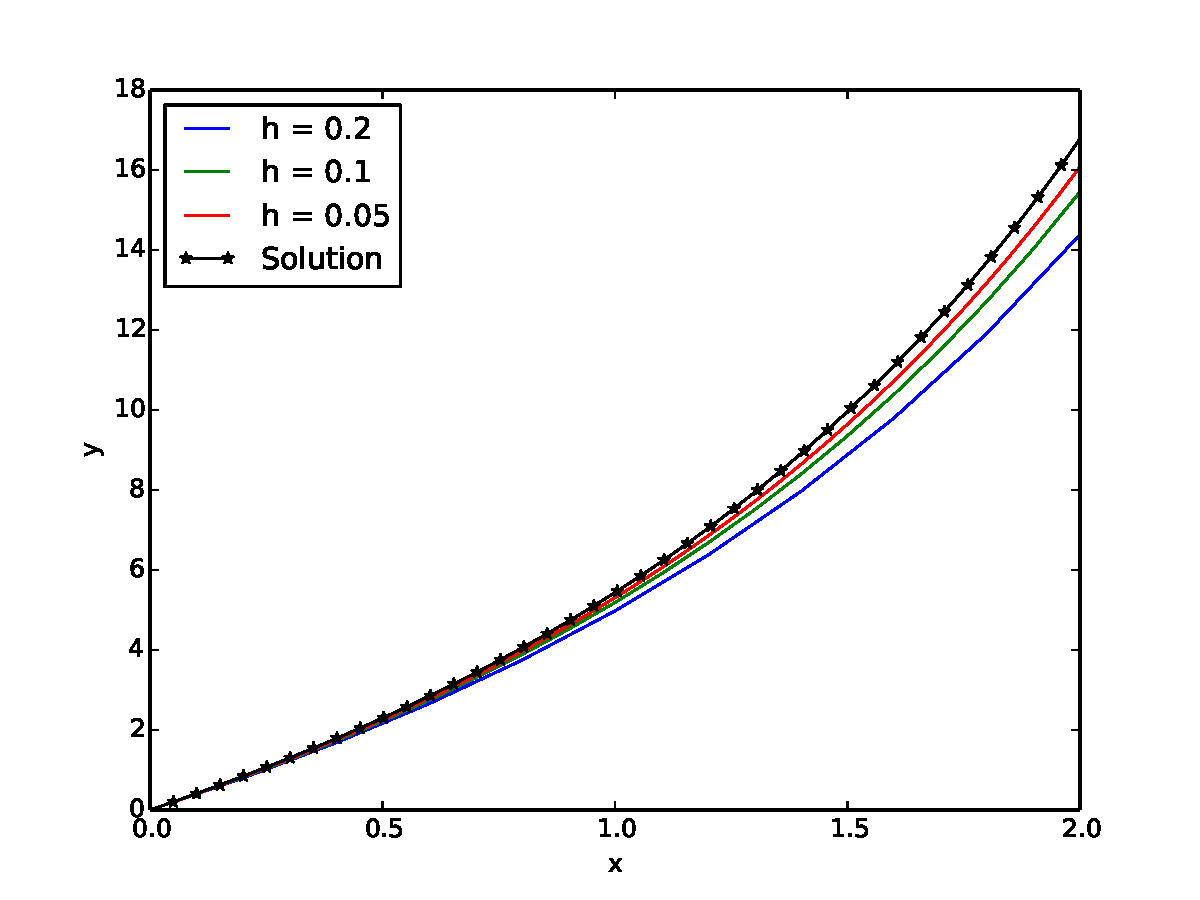
\includegraphics[width=\textwidth]{Fig1.pdf}
\caption{The solution of $y' -y= -2x+4, y(0) = 0$, is $y(x) = -2+2x + 2e^x.$ This is a plot of the solution, alongside approximations with Euler's method for several stepsizes.}
\label{ivp:euler}
\end{figure}


\begin{figure}[ht]
\centering
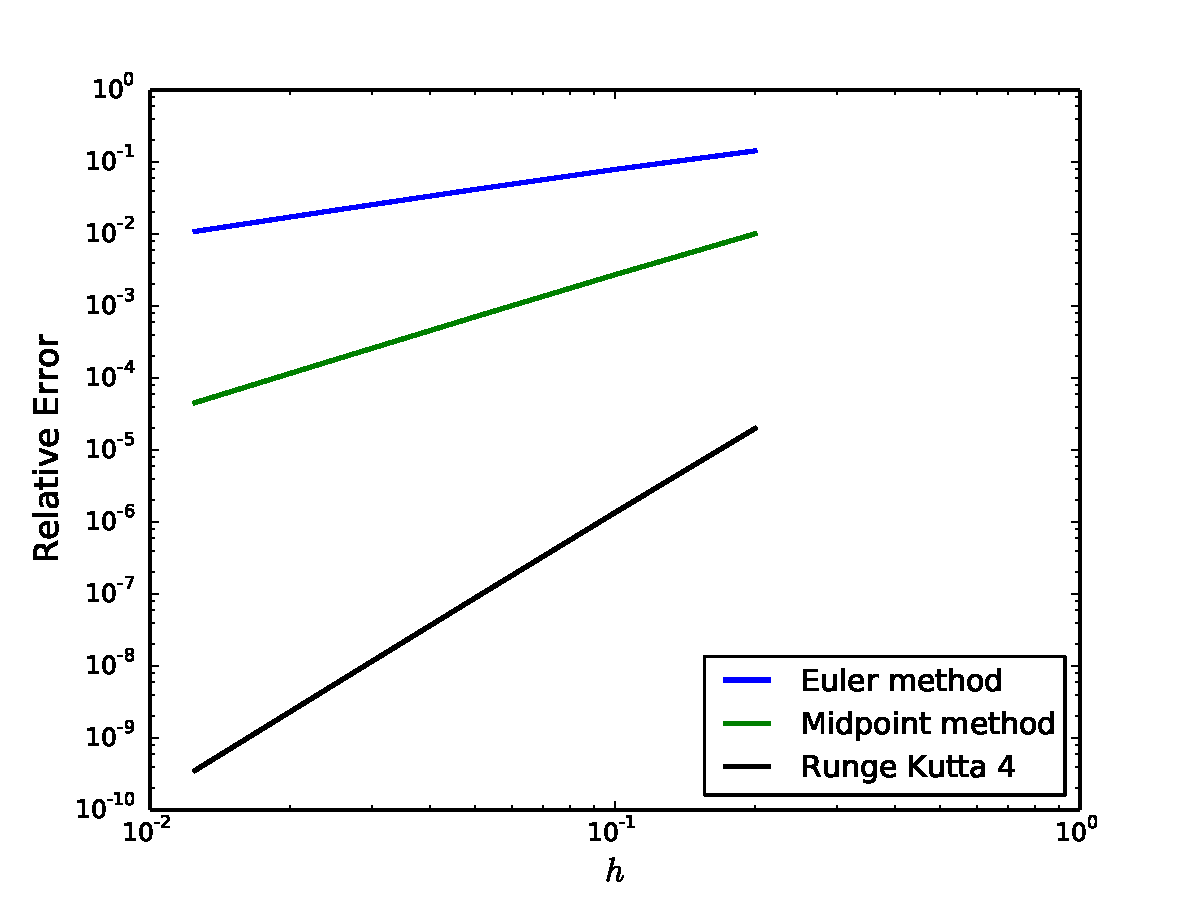
\includegraphics[width=\textwidth]{Fig3.pdf}
\caption{The solution of $y' -y= -2x+4,$ $ y(0) = 0$, is $y(x) = -2+2x + 2e^x.$ This is a loglog plot of the relative error in numerically approximating $y(2)$, using stepsizes $h = 0.2,$ $0.1,$ $0.05,$ $0.025,$ and $0.0125$. The plot shows first, second, and fourth order convergence for the Euler method, Midpoint method, and the RK4 method, respectively.}
\label{ivp:relative_error}
\end{figure}


\begin{problem} The solution of the IVP
\begin{align*}
y' + y &= 2-2x,\,\, 0 \leq x \leq 2, \\
y(0) &= 0,
\end{align*}
is given by $y(x) = 4-2x -4e^{-x}$. 
Use Euler's method to numerically approximate the solution with step sizes $h = 0.4, 0.2$, and $0.1.$ Plot your results.
\end{problem}


So how do we come up with numerical methods with higher order accuracy? Using Taylor's theorem (as we did for Euler's method) to create higher-order one-step methods would lead to numerically approximating derivatives of $f(t,y)$ - not necessarily desirable. 

Let us look for a second order method of the form 
\begin{enumerate}
\item $y_0 = y(a),$
\item $y_{i+1} = y_i + a f(x_i+b, y_i+c).$
\end{enumerate}


By expanding $a f(x+b, y+c)$ with Taylor's theorem and matching constants in the equation
\begin{align*}
f(x,y) + \frac{h}{2}f'(x,y) &= f(x,y) + \frac{h}{2}\frac{\partial f}{\partial x}(x,y) +  + \frac{h}{2}\frac{\partial f}{\partial y}(x,y) \cdot f(x,y),
\end{align*}
we find that $a = 1, b = h/2,$ and $c = h/2$. This method is called the Midpoint method. IVP solvers with this general form are called \textit{Runge-Kutta methods}. Another second order Runge-Kutta method is the modified Euler method: 

\begin{enumerate}
\item $y_0 = y(a)$,
\item $y_{i+1} = y_i + \frac{h}{2}[ f(x_i, y_i) + f(x_{i+1}, y_i+ hf(x_i, y_i))]$ for $i = 0,1,\hdots, n-1.$
\end{enumerate}


There are many Runge-Kutta methods with varying orders of accuracy. In practice, the methods of order four, such as the following, are most commonly used: 
\begin{enumerate}
\item $y_0 = y(a)$, 
\item $K_1 = hf(x_i,y_i),$
\item $K_2 = hf(x_i + \frac{h}{2}, y_i + \frac{1}{2} K_1),$
\item $K_3 = hf(x_i + \frac{h}{2} , y_i + \frac{1}{2} K_2),$
\item $K_4 = hf(x_{i+1} , y_i +  K_3),$
\item $y_{i+1} = y_i + \frac{1}{6}(K_1 + 2K_2 + 2K_3 + K_4)$ for $i = 0,1,\hdots,n-1.$
\end{enumerate}


\begin{problem}
Suppose a differential equation is given by
\[ y' = f(t).\]
Which quadrature formulas correspond to Euler's method, backward Euler's method, modified Euler's method, the Midpoint method, and the fourth order Runge-Kutta method (RK4)? 
\end{problem}



\begin{problem} Consider the IVP given by 
\begin{align*}
y' + y &= 2-2x,\,\, 0 \leq x \leq 2, \\
y(0) &= 0.
\end{align*}
Use Euler's method, the Midpoint method, and RK4 to approximate the value of the solution at $x = 2$, with a stepsize of $h = 0.2,$ $ 0.1,$ $0.05 $, $0.025,$ and $0.0125.$ Create a log-log plot of the relative error of each approximation using the \li{loglog} function in \li{matplotlib}.(see Figure \ref{ivp:relative_error}).
\end{problem}

% \begin{problem}
% Plot the solutions of 
% \[ y' + y = 2-2x\,\, 0 \leq x \leq 2, \] 
% with initial conditions $y(0) = 0, 2, 4, 6, $ and $8$. Use RK4 to compute the solutions. 
% \end{problem}

\pagebreak
\section{Harmonic Oscillators and Resonance} Harmonic oscillators show up often in classical mechanics. 
A few examples include the pendulum (with small 
 displacement), spring-mass systems, and the flow of electric current through various types of circuits. 
A harmonic oscillator can be described by an initial value problem of the form 
\begin{align*}
	my'' + \gamma y' + ky &= f(t) ,\\
	y(0) &= y_0,\\
	y'(0) &= y'_0.
\end{align*}

We will describe the construction of this mathematical model in the context of a spring-mass system.

Suppose an object with mass $m$ is placed at the end of a horizontal spring. 
The natural position of the object is called the \textit{equilibrium position} for the system.
If the object is displaced from its equilibrium position and given an initial velocity,  
it will act like a harmonic oscillator.
The principal property of a harmonic oscillator $y(t)$ is that once $y$ leaves its equilibrium value $y = 0$, it experiences a restoring force $F_r = -ky.$ 
This force pushes $y$ back towards its equilibrium. 
Hooke's law says that this holds true for a 
spring-mass system if the displacement $y$ is small.

Often there is an additional damping force $F_d$, often due to some type of friction. This force is usually proportional to the $y'$, is always in the opposite direction of $y'$, and represents energy leaving the system. 
Thus we have $F_d = -\gamma y', $ where $ \gamma \geq 0$ is constant. 
We may also need to consider an additional external force $f(t)$ that is interacting with our spring-mass system.

By using Newton's law we obtain
\begin{align*}
ma &= F = F_r + F_d + f(t),\\
my'' &= -ky -\gamma y' + f(t).
\end{align*}


\section*{Simple harmonic oscillators}
A simple harmonic oscillator is a harmonic oscillator that is not damped ($\gamma =0$), and is free ($f(t) \equiv 0$) rather than forced ($f(t) \not = 0$). A simple harmonic oscillator can described by the IVP
\begin{align*}
my'' + ky &= 0,\\
y(0) &= y_0,\\
y'(0) &= y_0'.
\end{align*} 
The solution of this IVP is $y = c_1\cos (\omega_0 t) + c_2 \sin (\omega_0 t)$ where $\omega_0 = \sqrt{k/m}$ is the natural frequency of the oscillator and $c_1$ and $c_2$ are determined by applying the initial conditions. This in turn can be written in the form 
\[y = A\sin (\omega_0 t + \delta) .\]

To solve this IVP using the fourth order Runge Kutta method (RK4), we need to write this system in the form 
\[z'(t) = f(t,z(t)) \]
We can do this by letting $z_1 = y, z_2 = y'$. Then we have \[     z'= 
 \left[\begin{array}{c}z_1 \\z_2\end{array}\right]'  =  \left[\begin{array}{c}z_2 \\\frac{k}{m}z_1\end{array}\right]= f(z).\]


\begin{problem} Use the RK4 method to solve for the simple harmonic oscillator 
described by 
\begin{align*}
my'' + ky &= 0,\,\, 0 \leq x \leq 20, \\
y(0) &= 2, \\
y'(0) &= -1,
\end{align*} 
for $m = 1$ and $k =1$. Note that in your implementation of RK4, the constants $K_1, K_2, K_3,$ and $K_4$ become vectors with $n$ entries, where $n$ is the number of equations in the first-order system. 

Plot your solution $y(t)$.  Compare this with the solution of the IVP if  $m = 3$ and $k =1$. Consider: Why does the difference in solutions make sense physically?
\end{problem}


\section*{Damped free harmonic oscillators} We now consider damped free harmonic oscillators. These systems are described by the differential equation
\[my''(t) +\gamma y'(t) + ky(t) = 0.\]
For fixed values of $m$ and $k$, it is interesting to study the effect of the damping coefficient $\gamma$. 

The roots of the characteristic equation are \[r_1,r_2 = \frac{-\gamma \pm \sqrt{\gamma^2 -4km}}{2m} .\]
Note that the real parts of $r_1$ and $r_2$ are always negative, and so any solution $y(t)$ will decay over time due to a dissipation of the system energy. There are several cases to consider for the general solution of this equation: 
\begin{enumerate}
\item If $\gamma^2 > 4km$, then the general solution is $y(t) = c_1 e^{r_1t} + c_2e^{r_2t}$. Here the system is said to be $\textit{overdamped}$. Notice from the general solution that there is no oscillation in this case.
\item If $\gamma^2 = 4km$, then the general solution is $y(t) = c_1 e^{\gamma t/2m} + c_2 te^{\gamma t/2m}$. Here the system is said to be $\textit{critically damped}$. 
\item If $\gamma^2 < 4km$, then the general solution is 
\begin{align*}
y(t) &= e^{-\gamma t/2m} \left[c_1\cos(\mu t) + c_2 \sin (\mu t)\right],\\
&= R e^{-\gamma t/2m}  \sin (\mu t + \delta),
\end{align*}
where $R$ and $\delta$ are fixed, and $\mu = \sqrt{4km-\gamma^2}/2m.$ This system does oscillate.
\end{enumerate}



\begin{problem}
Use RK4 method to solve for the damped free harmonic oscillator 
\begin{align*}
y'' +\gamma y'+ y &= 0, \,\, 0 \leq x \leq 20,\\
y(0) &= 1, \\
y'(0) &= -1.
\end{align*} 
For $\gamma = 1/2,$ and $\gamma = 1$, simultaneously plot the solutions $y(t)$ and find $y(20)$ accurate to four significant digits. (Check that the relative error is less than $5 \cdot 10^{-5}$.)  How many subintervals do you need?
\end{problem}





\section*{Forced harmonic oscillators without damping}
Let's look at the systems described by the differential equation
\begin{align}
my''(t)  + ky(t) &= F(t). \label{Forced_harm_osc}
\end{align}
In many instances the external force $F(t)$ is periodic, so let us assume that $F(t) = F_0 \cos(\omega t)$. If $\omega_0 = \sqrt{k/m} \not = \omega,$ then the  general solution of \ref{Forced_harm_osc} is given by 
\[y(t) = c_1 \cos (\omega_0 t) + c_2\sin (\omega_0 t) + \frac{F_0}{m(\omega_0^2 - \omega^2)} \cos (\omega t).\]
If $\omega_0 = \omega$, then the general solution is 
\[y(t) = c_1 \cos (\omega_0 t) + c_2\sin (\omega_0 t) + \frac{F_0}{2m\omega_0} t \sin (\omega_0 t).\]
This last solution contains a term that grows arbitrarily large as $t \to \infty$. 
If we included damping then the solution would be bounded, but will still be large for small $\gamma$ and $\omega$ close to $\omega_0$. 
Let us consider physical spring-mass system. 
Equation \ref{Forced_harm_osc} holds only for small oscillations (this is where Hooke's law is applicable). 
For larger oscillations, this equation will not hold. 
However, the fact that the equation predicts large oscillations suggests the spring-mass system could fall apart as a result of the external force. Mechanical resonance has 
been known to cause failure of bridges, buildings, and airplanes.



\begin{problem}
Use the RK4 method to solve for the undamped forced harmonic oscillator
\begin{align*}
2y'' + \gamma y' + 2y &= 2 \cos (\omega x), \,\, 0 \leq x \leq 40,\\
y(0) &= 2, \\
y'(0) &= -1.
\end{align*} 
For the following values of $\gamma$ and $\omega,$ plot the solution $y(t)$ and find $y(40)$ correct to four decimal places: 
\begin{align*}
	(\gamma, \omega) &= (0.5, 1.5),\\
	 &= (0.1, 1.1), \\
	&= (0.0, 1.0).
\end{align*}
\end{problem}


